\section{Quantum Annealing}
In this section we report on our efforts to solve problem instances from the departure delay model from section \ref{sec:departure_delay_model} with a D-Wave 2X quantum annealer.
We restricted ourselves to instances with $d_\text{max}=D_\text{max}=18$ and $\Delta_d \in \{3, 6, 9\}$.
\subsection{Embedding}
In order to make a QUBO amenable for a D-Wave 2X quantum annealer, it has to obey certain hardware constraints.
For instance the connections between the binary variables are restricted to the so called Chimera graph \footnote{Reference to Chimera graph}.
However, it is possible to map every QUBO to another QUBO which obeys the Chimera architecture while increasing the number of binary variables used by a so called minor-embedding technique \footnote{Reference to minor-embedding}. 

\begin{table}[htpb]
    \begin{tabular}{lrrr}
    \toprule
    $\Delta_d$ &    3 &    6 &    9 \\
    \midrule
    Number of flights $N_f$   &   13 &   19 &   50 \\
    Number of conflicts $N_c$ &   27 &   47 &  104 \\
    Number of logical qubits  &   91 &   76 &  150 \\
    Average number of physical qubits &  631 &  395 &  543 \\
    \bottomrule
    \end{tabular}
    \caption{Parameters of the largest embeddable instances for the D-Wave 2X}
    \label{tab:embedding}
\end{table}

We found, that non of the instances were suitable for direct calculation on the D-Wave machine.
Therefore we used D-Wave's heuristic embedding algorithm \footnote{Reference to D-Wave embedding algorithm} to embed instances with up to $N_f=50$ and $N_c=104$ depending on discretization (cf.\ table \ref{tab:embedding}).
In figure \ref{fig:number_of_physical_qubits} on can see the dependence of the number of physical qubits on the number of logical qubits.


\begin{figure}[htpb]
    \centering
    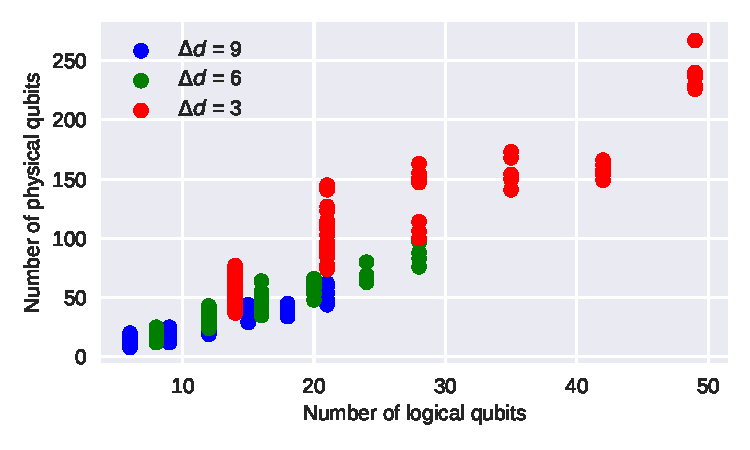
\includegraphics[width=0.45\textwidth]{./pics/physicalVsLogicalNumberOfQubits.pdf}
    \caption{Number of physical qubits versus the number of logical qubits after embedding of QUBO instances for the departure delay model.}
    \label{fig:number_of_physical_qubits}
\end{figure}


\subsection{Success Probability}
In order to investigate the performance of the D-Wave 2X machine, we compared its results to the ones of an exact solver.
We used an exact Max-SAT solver~\cite{TODO:akmaxsat} after we mapped the QUBOs to Max-SAT~\cite{TODO:reference-for-QUBO-to-MAXSAT-mapping}.
For each QUBO instance, we ran the annealing process $N_r = 10000$ times. 
The success probability is then given by the ratio of the number of annealing solutions which are equal to exact solution and the $N_r$.

\begin{figure}[htpb]
    \centering
    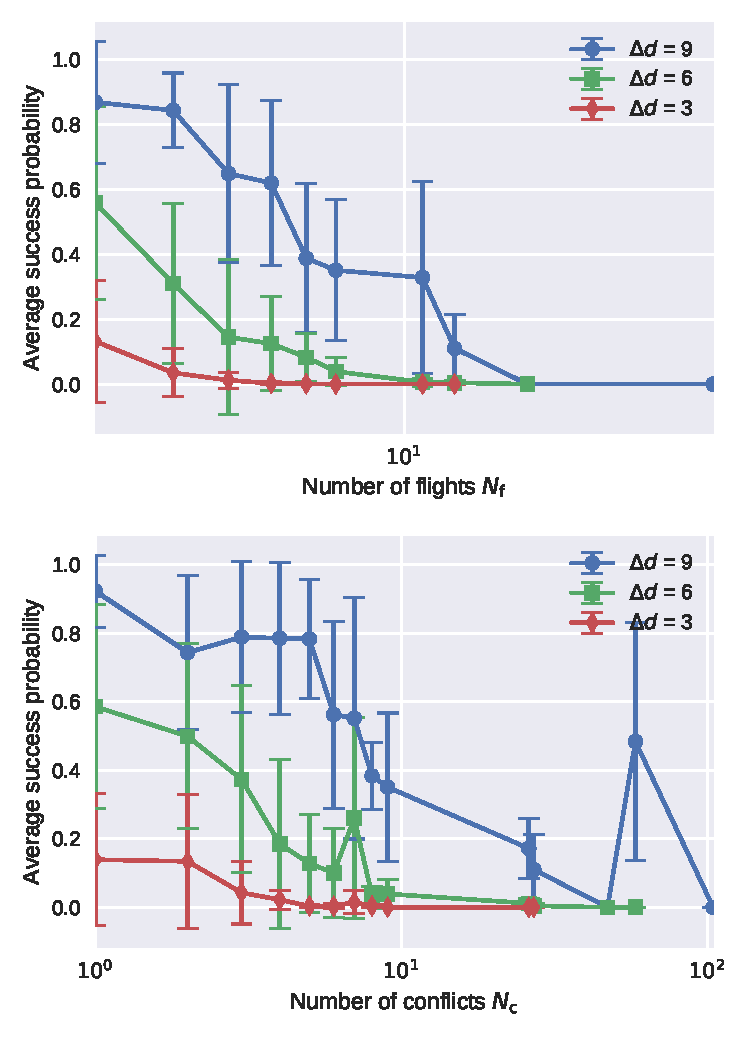
\includegraphics[width=0.45\textwidth]{./pics/annealing_results_success_vs_flights_and_conflicts.pdf}
    \caption{Average success probability for QUBO instances in dependence of the number of flights $N_f$ and the number of conflicts $N_c$. 
             The error bars indicate the standard deviation.
             We used $10000$ annealing runs for each instance and penalty weights $\lambda = \lambda_\text{conflict} = \lambda_\text{unique} \in \{0.5, 1, 2\}$. 
    }
\label{fig:success_probability}
\end{figure}

In figure~\ref{fig:success_probability} the dependence of the average success probability on the number of flights and the number of conflicts is shown.
The average was taken over all successfully embedded QUBO instances with the same number of flights and number of conflicts, respectively.
On can see, that the success probability decreases for larger problem instances as well as for finer discretizations. 
This is a result of the limited precision in the specification of a QUBO on the D-Wave 2X machine~\cite{TODO:D-Wave-precision}.



